\documentclass[mathserif]{beamer}

\usepackage{tikz}
\usetikzlibrary{calc}

\providecommand{\rowvisible}[4]{
  \visible<#1>{#2} & \visible<#1>{#3} & \visible<#1>{#4}
}

\begin{document}
\begin{frame}
  \begin{columns}
    \begin{column}{0.45\linewidth}
      \begin{figure}
        \centering
        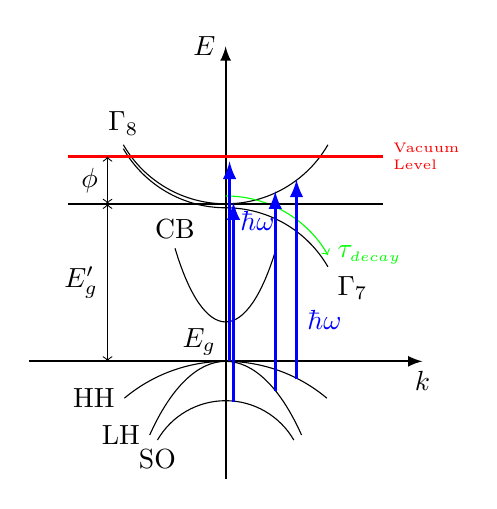
\begin{tikzpicture}
  % grid
  %\draw (-3,-2) grid (3,5);

  % axes
  \draw [-latex, thick] (-2.5,0) -- (2.5,0) node [below] {$k$};
  \draw [-latex, thick] (0,-1.5) -- (0,4) node [left] {$E$};

  % bands
  %\draw (-1,-0.5) .. controls (-0.25,0.25) .. (0,0);
  %\draw (-1,-1) .. controls (-0.5,0) and (0.5,0) .. (1,-1);
  \coordinate (so gamma) at (0,-0.5);
  \draw<3-> (so gamma) arc [start angle=90, end angle=30,  radius=1];
  \draw<3-> (so gamma) arc [start angle=90, end angle=150, radius=1]
    node [below] {SO};

  \coordinate (origin) at (0,0);
  \draw (origin) arc [start angle=90, end angle=50,  radius=2];
  \draw (origin) arc [start angle=90, end angle=130, radius=2]
    node [left] {HH};

  \draw (origin) arc [start angle=90, end angle=50,  x radius=1.5, y radius=4];
  \draw (origin) arc [start angle=90, end angle=130, x radius=1.5, y radius=4]
    node [left] {LH};

  \coordinate (cb gamma) at (0,0.5);
  \draw (cb gamma) arc [start angle=-90, end angle=-50,  x radius=1, y radius=4];
  \draw (cb gamma) arc [start angle=-90, end angle=-130, x radius=1, y radius=4]
    node [above] {CB};
  \node [left] at ($(cb gamma)!0.5!(origin)$) {$E_g$};

  \coordinate (gamma 8) at (0,2);
  \draw<2-> (gamma 8) arc [start angle=-90, end angle=-30,  radius=1.5];
  \draw<2-> (gamma 8) arc [start angle=-90, end angle=-150, radius=1.5]
    node [above] {$\Gamma_{8}$};

  \coordinate (gamma 7) at (0,1.95);
  \draw<7-> (gamma 7) arc [start angle=90,  end angle=30,   radius=1.5]
    node [below right] {$\Gamma_{7}$};
  \draw<7-> (gamma 7) arc [start angle=-90, end angle=-150, radius=1.5];
  \draw<7-> [green,->] (gamma 7) ++(0,0.15) arc [start angle=90,  end angle=30,   radius=1.5]
    node [right] {$\tau_{{\scriptscriptstyle decay}}$};

  % defined energies
  \coordinate (energies) at (-1.5,0);
  \draw<4-> [thick] ($(gamma 8) + (-2,0)$) -- ++(4,0);
  \draw<4-> [<->] (energies) -- (energies |- gamma 8)
    node [pos=0.5,left] {$E_{g}^{\prime}$};

  \coordinate (vacuum level) at ($(gamma 8) + (0,0.6)$);
  \draw [thick,red] ($(vacuum level) + (-2,0)$) -- ++(4,0)
    node [right,align=left,font=\tiny] {Vacuum\\Level};
  \draw<4-> [<->] (energies |- gamma 8) -- (energies |- vacuum level)
    node [pos=0.5,left] {$\phi$};

  % photon excitation
  \draw<1> [-latex, blue, very thick] (0.05,0) -- ++(0,2.54)
    node [right,pos=0.7] {$\hbar \omega$};
  \draw<3-> [-latex, blue, very thick] (0.1,-0.52) -- ++(0,2.54);
  \draw<2-> [-latex, blue, very thick] (0.63,-0.38) -- ++(0,2.54);
  \draw<2-> [-latex, blue, very thick] (0.9,-0.23) -- ++(0,2.54)
    node [right,pos=0.3] {$\hbar \omega$};

\end{tikzpicture}

      \end{figure}
    \end{column}
    \begin{column}{0.53\linewidth}
      \begin{tabular}{|c|c|c|}
        \hline
          & GaSb & InSb \\ \hline
        \rowvisible{4-}{$E_{g}^{\prime}$}{3.77eV}{3.59eV} \\ \hline
        \rowvisible{4-}{$\phi$}{0.99eV}{1.18eV} \\ \hline
        \rowvisible{5-}{Excess $E$}{$\sim$0.35eV}{$\sim$0.41eV} \\
        \rowvisible{5-}{$\Rightarrow$ initial $T_e$}{4200K}{4900K} \\ \hline
        \rowvisible{8-}{$m^{*}(\Gamma_8)$}{$0.3 m_0$}{$0.5 m_0$} \\ \hline
      \end{tabular}
      \vphantom{X}\\
      \visible<6->{
        $\exp(-\phi / k_{{\scriptscriptstyle B}} T_e) \approx 0.6$
        \begin{itemize}
          \item thermionic photoemission!
        \end{itemize}
      }
      \visible<7->{
        Cooling rates of $\sim$1600 K/ps from
        \begin{itemize}
          \item LO phonons 
          \item fast decay via $\Gamma_7$
        \end{itemize}
      }
    \end{column}
  \end{columns}
\end{frame}
\end{document}
